\documentclass{article}

\usepackage[letterpaper]{geometry}
\usepackage[T1]{fontenc}
\usepackage[utf8]{inputenc}
\usepackage[english]{babel}
\usepackage{csquotes}
\usepackage{latexsym, amsmath,amssymb}
\usepackage{graphicx}
\usepackage{subcaption}
\usepackage{booktabs,multicol}
\usepackage[table]{xcolor}

% easy author affiliations
\usepackage{authblk}
\renewcommand\Affilfont{\small}

\usepackage[hyphens]{url}
\usepackage[breaklinks=true,linkcolor=blue, citecolor=blue, urlcolor=blue, colorlinks=true]{hyperref}

\usepackage[
    backend=biber,
    style=numeric,
    citestyle=numeric-comp,
    sorting=none,
    bibencoding=UTF-8,
    giveninits=true,
    maxbibnames=1000,
]{biblatex}
\addbibresource{references.bib}

\usepackage{todonotes}

\hyphenation{NumFOCUS}

\newcommand\joss{\textit{JOSS}}

\title{Publish your software: introducing the Journal of Open Source Software (JOSS)}

\author[1]{Daniel S.~Katz\thanks{Corresponding author, \href{mailto:d.katz@ieee.org}{d.katz@ieee.org}}}
\author[2]{Kyle E.~Niemeyer}
\author[3]{Arfon M.~Smith}
%\author{\textcolor{red}{any other JOSS editors as authors?}}

\affil[1]{National Center for Supercomputing Applications \& Department of Computer Science \& Department of Electrical and Computer Engineering \& School of Information Sciences, University of Illinois Urbana--Champaign, Urbana, IL, USA}
\affil[2]{School of Mechanical, Industrial, and Manufacturing Engineering, Oregon State University, Corvallis, OR, USA}
\affil[3]{Space Telescope Science Institute, Baltimore, MD, USA}

\date{6 February 2018}

\begin{document}

\maketitle

%\noindent \textcolor{red}{Based on \href{https://www.sharelatex.com/project/599496d1d932c809895dc1cd}{PeerJ paper submission} \\ CiSE wants 2K-4K words (with figures counting for 250 words).  2 pages of LaTeX full text is about 500 words, so this is about 4-8 pages here, minus 1 page per figure.  I imagine we should also not have many references, so I've put some URLs in-line}

\section{Motivation}

Software is essential to most research today. We know this because we have asked researchers, and we have examined their outputs.
%
A 2014 study of UK Russell Group Universities~\cite{Hettrick} reports that about 90\% of academics surveyed said they use software in their research, while more than 70\% said their research would be impractical without it.  
About half of these UK academics said they develop their own software while in the course of doing research.
Similarly, a 2017 survey of members of the US National Postdoctoral Association found that 95\% used research software, and 63\% said their research would be impractical without it~\cite{US-PDA-survey}.
%
The initial phases of a study of the role of software in journal articles began with examining three months of the journal \textit{Nature}.
In these three months, there were 40 research articles, and of these, 32 included mentions of software, and averaged 6.5 software packages mentioned per article~\cite{nature-survey}.


However, even though software is a critical part of modern research, software publication, acknowledgement, and citation are not well-supported across the scholarly ecosystem~\cite{Niemeyer:2016sc}. 
Academic publishing has not changed substantially since its inception.
Science, engineering, and many other academic fields still view research articles as the key indicator of research productivity, with research grants being another important indicator.
Yet, the research article is inadequate to fully describe modern, data-intensive, computational research. 

\textit{The Journal of Open Source Software} (\joss{}, \href{http://joss.theoj.org}{joss.theoj.org}) \cite{joss-peerj} focuses on research software and its place in the scholarly publishing ecosystem. Its goal is to make it easy for authors to publish a paper about their software, mostly focused on the software itself, and then to be able to get credit when this software is used based on the users citing the \joss{} paper. Its selling point for authors is:

\begin{center}
\vspace{0.1cm}
\noindent\fbox{%
    \parbox{0.85\textwidth}{%
        ``If you've already licensed your code and have good documentation then we expect that it should take less than an hour to prepare and submit your paper to JOSS.''
    }%
}
\end{center}
\vspace{0.1cm}

\joss{} is:
\begin{itemize}

\item Built on GitHub: We use GitHub so that we can take advantage of numerous GitHub features (the use of issues for reviews; rapid interaction between author, reviewer, and editor; notifications) and the general familiarity of  both authors and reviewers with GitHub.

\item Open access: Papers submitted to and accepted by \joss{} are open access(CC-BY licensed), and authors retain the copyright of their work. The software components of the publications are licensed under an OSI-approved license. 

\item Intended for research software: \joss{} attempts to be general to all research software, not just for science or any single field.  The main question \joss{} asks of submitters is: ``Is it likely that users of this software will want to cite it?''

\item Intended to be easy-to-use for authors: Authors with well-documented code in a public code repository just need to create a directory in that repository that contains a short paper in markdown format, and in that paper, declare the authors of the software, the purpose of the software, and any needed references. 

\item Intended to be easy-to-use for reviewers: Reviewers just need to work through a checklist of items related to the \joss{} conflicts of interest policy, the code and documentation in the software repository, and the software paper itself, as further discussed in Section~\ref{sec:process}.

\item Supported by NumFOCUS: NumFOCUS (\href{https://www.numfocus.org}{numfocus.org}) is a 501(c)(3) nonprofit that supports and promotes world-class, innovative, open source scientific computing. It provides a forum for such projects to work through issues, and provides a mechanism for these projects to accept funding. Open Journals\footnote{\url{http://theoj.org}} is a collection of open source, open access journals, of which, \joss{} is the flagship publication. Other journals based on the same (\joss{}) model are in varying stages of spinning up.

\item Endorsed and affiliated with the Open Source Initiative: The OSI (\href{https://opensource.org}{opensource.org}) is a global non-profit that protects and promotes open source software, development and communities, championing software freedom in society through education, collaboration, and infrastructure, stewarding the Open Source Definition (OSD), and preventing abuse of the ideals and ethos inherent to the open source movement. In support of this mission, \joss{} requires that the  software it publishes uses an OSI-approved license.

\item Indexed. \joss{} is listed on Sherpa/Romeo, and \joss{} papers are indexed by ADS\footnote{\url{http://adsabs.harvard.edu}}, which in turn is indexed by Google Scholar.

\item Connected to other code reviewing systems: For submissions of software that has already been reviewed under rOpenSci's rigorous
onboarding guidelines~\cite{Ram:2016ws}, \joss{} does not perform 
further review; the editor-in-chief fast-tracks such submissions to acceptance. And this could be extended to work with other trustworthy systems.

\end{itemize}


\section{\joss{} process}\label{sec:process}

The typical \joss{} submission and review process (shown in Figure~\ref{fig:submission-flow}) is: 

\begin{enumerate}
\item An author submits an article, including a link to software, to \joss{} using the web application and submission tool.
The article is a Markdown file named \texttt{paper.md}, visibly located in the software repository (in many cases, placed together with auxiliary files in a \texttt{paper} directory).

\item Following a routine check by a \joss{} administrator, a ``pre-review'' issue is created in the \texttt{joss-reviews}\footnote{\url{https://github.com/openjournals/joss-reviews}} GitHub repository. In this pre-review issue, an editor is assigned, who then identifies and assigns a suitable reviewer. The editor then asks the automated bot \texttt{Whedon} to create the main submission review issue.

\item The reviewer then conducts the submission review in the issue by working through a checklist of review items:

\begin{itemize}
\item Agreement with \joss{} policies on conflicts of interest and code of conduct.
\item General checks on source code availability, use of an OSI-approved license, match of the software version in the paper and the repository, and that the submitter is an author of the software.
\item Checks on functionality, including installation and performance claims, if appropriate.
\item Checks on documentation, which should include a statement of need for the software, installation instructions, example usage, and documentation of functionality, tests, and community guidelines.
\item Checks on the software paper itself, including ensuring that the list of authors is reasonable, the statement of need is in the paper, and that sufficient and well-structured references are present.
\end{itemize}

The author, reviewer, and editor discuss any questions that arise during the review, and once the reviewer completes their checks, they notify the submitting author and editor. 
\joss{} reviews are discussions---in the open within a GitHub issue---between the reviewer(s), author(s), and editor. 
Like a true conversation, discussion can go back and forth in minutes or seconds, with all parties contributing at will. This contrasts with traditional journal reviews, where the process is merely an exchange between the reviewer(s) and author(s) via the editor, which can take months for each communication, and in practice is usually limited to one to three exchanges due to that delay~\cite{tennant-peerreview}.
The reviews are subject to a code of conduct (\href{https://github.com/openjournals/joss/blob/master/CODE_OF_CONDUCT.md}{CODE\_OF\_CONDUCT.md}); both authors and reviewers must confirm that they have read and will adhere to this Code of Conduct, during submission and with their review, respectively.

\item After the review is complete, the editor asks the submitting author to make a permanent archive of the software (including any changes made during review) with a service such as Zenodo or Figshare, and to post a link to the archive in the review thread. This link, in the form of a DOI, is attached to the submission.

\item The editor-in-chief produces a compiled PDF, updates the \joss{} website, deposits Crossref metadata, and issues a Crossref DOI for the submission. 

\item Finally, the editor-in-chief updates the review issue with the \joss{} article DOI and closes the review. The submission is then accepted into the journal.

\end{enumerate}
\begin{figure}[htp]
\centering
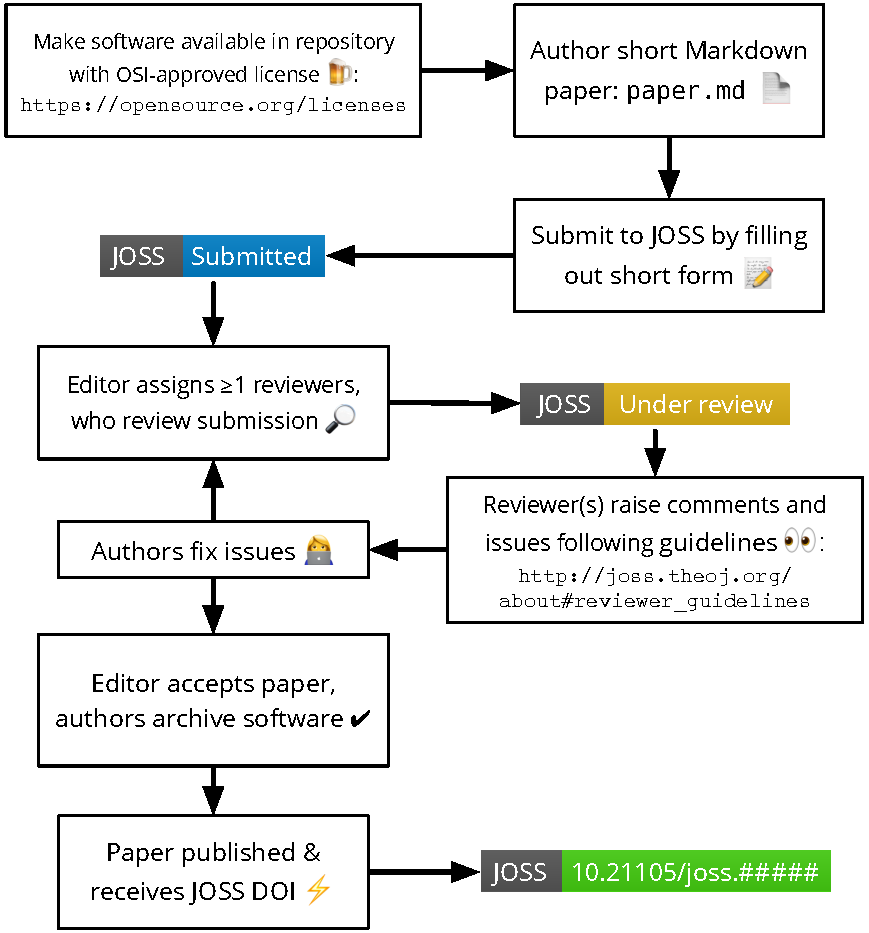
\includegraphics[width=0.75\textwidth]{JOSS-flowchart.pdf}
\caption{The \joss{} submission and review flow including the various status badges that can be embedded on third-party settings such as GitHub README documentation~\cite{JOSS-publication-workflow}.
\label{fig:submission-flow}}
\end{figure}


\section{Status and future directions}

\joss{} received its first submission in May 2016, and as of January 22, 2018, it has published 206 papers, and has 63 more that have been submitted and are being reviewed or otherwise processed.
The most-cited \joss{} articles in the first almost 20 months are \texttt{corner.py}~\cite{cornerpy} and \texttt{Armadillo}~\cite{armadillo}, with 129 and 86 citations, respectively, according to Google Scholar.

This and the fact that we have 19 volunteer editors seem to indicate that \joss{} is satisfying a need.  \joss{} is not the final answer for the problem we ultimately want to solve---we want authors to get credit for software directly; they should not need to write papers about their software to advertise it and to fit within the journal system---but it is a good intermediate step to highlight the need for recognition and credit for software.

As general awareness of \joss{} in the community increases, the \joss{} editorial team has received a number of expressions of interest from other journals and publishers who are interested in the \joss{} approach. These journals are generally either interested in 1) accepting software papers in their journals but want a deeper review of the software or 2) want to add software reviews to their editorial process for scientific papers but don't have the expertise in their reviewer pool. The approach being considered is to allow other journals to request a \joss{} review as part of their editorial process when software forms a major part of a submission. One example of a publisher interested in this approach is the American Astronomical Society (AAS) who has the high profile Astrophysical Journal (ApJ) among their publications.

In addition to potential collaborations with other journals, we are in the process of generalizing the \joss{} infrastructure to allow for other journals to be easily created using the same tools. Supported by a small grant from the Alfred P.\ Sloan Foundation, the core \joss{} application\footnote{\url{https://github.com/openjournals/joss}} and the \textit{Whedon}\footnote{\url{https://github.com/openjournals/whedon-api}} bot are being adapted to support multiple \joss{}-like publications. Led by a subset of the \joss{} editorial team, the \textit{Journal of Open Source Education} is likely to be the first new publication to use the generalized infrastructure.

\printbibliography

\end{document}
